\documentclass{article}
\usepackage{amsmath}
\usepackage{amssymb}
\usepackage{ctex}
\usepackage{graphicx}
\begin{document}
\title{�ڰ˴���ҵ}
\maketitle
1.$(2x)^2+(3y)^2=1$\\
\begin{figure}[!h]
  \centering
  % Requires \usepackage{graphicx}
  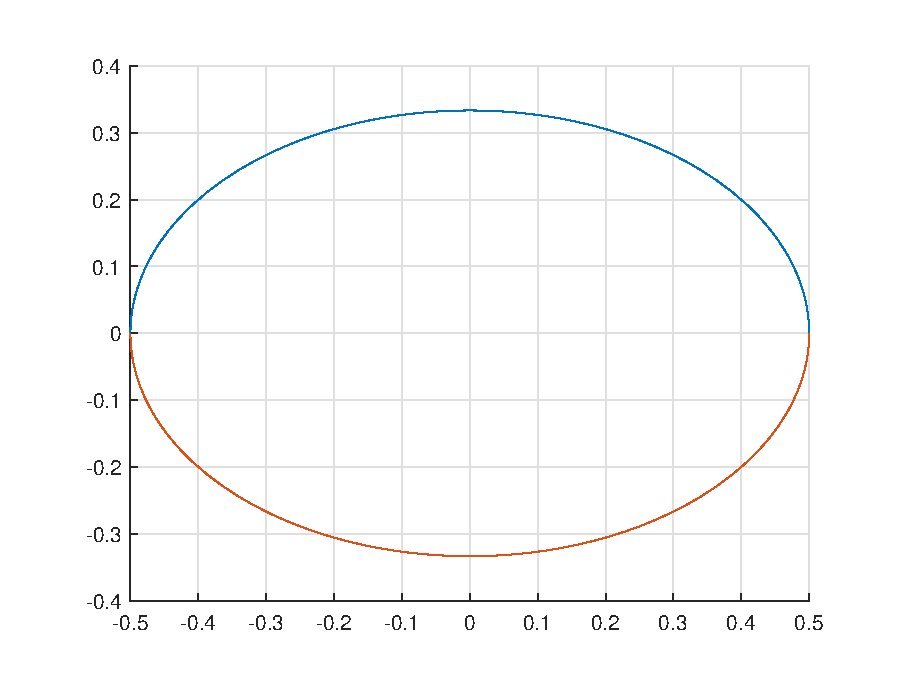
\includegraphics[scale=0.7]{8_1.eps}\\
  \caption{$(2x)^2+(3y)^2=1$}
\end{figure}\\
2.\[F\left[ \begin{gathered}
  x \hfill \\
  y \hfill \\
\end{gathered}  \right] = \left[ \begin{gathered}
  xy \hfill \\
  y \hfill \\
\end{gathered}  \right] \Rightarrow F\left[ \begin{gathered}
  2 \hfill \\
  y \hfill \\
\end{gathered}  \right] = \left[ \begin{gathered}
  2y \hfill \\
  y \hfill \\
\end{gathered}  \right]\]
\begin{figure}[!h]
  \centering
  % Requires \usepackage{graphicx}
  \includegraphics[scale=0.7]{8_2.eps}\\
\end{figure}\\
3.\[\begin{gathered}
  F(v) = F({a_1}{v_1} + {a_2}{v_2} +  \cdots {a_n}{v_n}) = {a_1}F({v_1}) + {a_2}F({v_2}) +  \cdots {a_n}F({v_n}) \hfill \\
  {\text{if }}F({v_j})(1 \leqslant j \leqslant n){\text{ is already known}} \hfill \\
  {\text{from one - to - one we can know that }}F{\text{ is uniquely defined}} \hfill \\
  {\text{if }}F{\text{ is not a linear mapping,we can't conclude that }}F{\text{ is uniquely defined}} \hfill \\
\end{gathered} \]
4.\[\begin{gathered}
  T(x + y) = T(x) + T(y) = 0 \hfill \\
  T(kx) = kT(x) = 0 \hfill \\
   \Rightarrow x + y \in V,kx \in V \hfill \\
  {\text{so }}\{ x \in V|T(x) = 0\} {\text{ is a subspace of }}V \hfill \\
\end{gathered} \]
5.\[\begin{gathered}
  (1)T(A + B) = \frac{{A + B + {A^T} + {B^T}}}{2} = \frac{{A + {A^T}}}{2} + \frac{{B + {B^T}}}{2} = T(A) + T(B) \hfill \\
  T(kA) = \frac{{kA + k{A^T}}}{2} = kT(A) \hfill \\
  {\text{so }}T{\text{ is a linear mapping}} \hfill \\
  (2)T(A) = 0 \Rightarrow \frac{{A + {A^T}}}{2} = 0 \Rightarrow A + {A^T} = 0 \hfill \\
  {\text{so the kernel of T consists in the linear space of all skew symmetric matrix}} \hfill \\
  {\text{(3)}}\forall A \in {\text{symmetric matrix,we can find countless matrices }}B \hfill \\
  A = \frac{{B + {B^T}}}{2} = T(B),{\text{so the range of  T consists in the linear space of all symmetric matrices}}{\text{.}} \hfill \\
  {\text{(4)the dimension of symmetric matrices is n}} \hfill \\
  {\text{if n is an odd number,}} \hfill \\
  {\text{then the dimension of skew symmetric matrices is n-1}} \hfill \\
  {\text{if n is an even number,}} \hfill \\
  {\text{then the dimension of skew symmetric matrices is n}} \hfill \\
\end{gathered} \]
6.\[\begin{gathered}
  (1)\left\{ \begin{gathered}
  x = 0 \hfill \\
  x - y = 0 \hfill \\
  x - z = 0 \hfill \\
  x - y - z = 0 \hfill \\
\end{gathered}  \right. \Rightarrow \left\{ \begin{gathered}
  x = 0 \hfill \\
  y = 0 \hfill \\
  z = 0 \hfill \\
\end{gathered}  \right. \hfill \\
  {\text{so the kernel of F is }}\left[ \begin{gathered}
  0 \hfill \\
  0 \hfill \\
  0 \hfill \\
\end{gathered}  \right] \hfill \\
  (2)F\left[ \begin{gathered}
  x \hfill \\
  y \hfill \\
  z \hfill \\
\end{gathered}  \right] = \left[ \begin{gathered}
  x \hfill \\
  x - y \hfill \\
  x - z \hfill \\
  x - y - z \hfill \\
\end{gathered}  \right] = x\left[ \begin{gathered}
  1 \hfill \\
  1 \hfill \\
  1 \hfill \\
  1 \hfill \\
\end{gathered}  \right] - y\left[ \begin{gathered}
  0 \hfill \\
  1 \hfill \\
  0 \hfill \\
  1 \hfill \\
\end{gathered}  \right] - z\left[ \begin{gathered}
  0 \hfill \\
  0 \hfill \\
  1 \hfill \\
  1 \hfill \\
\end{gathered}  \right] \hfill \\
  {\text{so the range of }}F{\text{ is }}{R^3} \hfill \\
\end{gathered} \]
7.\[\begin{gathered}
  T\left[ \begin{gathered}
  1{\text{ 0 0}} \hfill \\
  {\text{0 1 0}} \hfill \\
  {\text{0 0 1}} \hfill \\
\end{gathered}  \right] = \left[ \begin{gathered}
  1{\text{ 0 0}} \hfill \\
  {\text{0 1 0}} \hfill \\
  {\text{0 0 1}} \hfill \\
\end{gathered}  \right]\left[ \begin{gathered}
  1{\text{ 0 0}} \hfill \\
  {\text{0 2 0}} \hfill \\
  {\text{0 0 3}} \hfill \\
\end{gathered}  \right] \hfill \\
  T\left( {\begin{array}{*{20}{c}}
  {\frac{1}{{\sqrt 2 }}}&{\frac{1}{{\sqrt 2 }}}&0 \\
  {\frac{1}{{\sqrt 2 }}}&{\frac{1}{{\sqrt 2 }}}&0 \\
  0&0&{ - 1}
\end{array}} \right) = \left( {\begin{array}{*{20}{c}}
  {\frac{1}{{\sqrt 2 }}}&{\frac{1}{{\sqrt 2 }}}&0 \\
  {\frac{1}{{\sqrt 2 }}}&{\frac{1}{{\sqrt 2 }}}&0 \\
  0&0&{ - 1}
\end{array}} \right)\left( {\begin{array}{*{20}{c}}
  {{a_{11}}}&{{a_{12}}}&{{a_{13}}} \\
  {{a_{21}}}&{{a_{22}}}&{{a_{23}}} \\
  {{a_{31}}}&{{a_{32}}}&{{a_{33}}}
\end{array}} \right) \hfill \\
  \left( {\begin{array}{*{20}{c}}
  {{a_{11}}}&{{a_{12}}}&{{a_{13}}} \\
  {{a_{21}}}&{{a_{22}}}&{{a_{23}}} \\
  {{a_{31}}}&{{a_{32}}}&{{a_{33}}}
\end{array}} \right) = \left( {\begin{array}{*{20}{c}}
  {\frac{3}{2}}&{\frac{1}{2}}&0 \\
  {\frac{1}{2}}&{\frac{3}{2}}&0 \\
  0&0&3
\end{array}} \right) \hfill \\
  {\text{so the matrix associated with T under }}{v_1},{v_2},{v_3}{\text{ is }}\left( {\begin{array}{*{20}{c}}
  {\frac{3}{2}}&{\frac{1}{2}}&0 \\
  {\frac{1}{2}}&{\frac{3}{2}}&0 \\
  0&0&3
\end{array}} \right) \hfill \\
\end{gathered} \]
\end{document}
